\documentclass[letterpaper]{article}

\usepackage{ifthen}
\usepackage{xparse}
\usepackage{enumitem}
\usepackage[utf8]{inputenc}
\usepackage{amsmath}
\usepackage{amssymb}
\usepackage{stmaryrd}
\usepackage{amsthm}
\usepackage{mathtools}
\usepackage{proof}
\usepackage{colonequals}
\usepackage{comment}
\usepackage{textcomp}
\usepackage[us]{optional}
\usepackage{color}
\usepackage{url}
\usepackage{verbatim}
\usepackage{graphics}
\usepackage{mathpartir}
\usepackage{tikz}
\usepackage{todonotes}

% these two are used to create the wavy division sign
\usepackage{stackengine}
\usepackage{scalerel}

\usepackage{hyperref}
\usepackage[nameinlink, capitalise]{cleveref}

\usepackage{array}


%% Beamer defines a range of its own theorems
\ifx\beamer\undefined

\theoremstyle{plain}
\newtheorem{theorem}{Theorem}[section]
\newtheorem{lemma}[theorem]{Lemma}
\newtheorem{corollary}[theorem]{Corollary}

\theoremstyle{definition}
\newtheorem*{remark}{Remark}
\newtheorem*{notation}{Notation}
\newtheorem{definition}{Definition}
\newtheorem{conjecture}{Conjecture}
\newtheorem{example}{Example}

\else 
  %% Intentionally left blank
\fi

\makeatletter
\newcommand\xlabel[2][]{\phantomsection\def\@currentlabelname{#1}\label{#2}}
\makeatother

\newenvironment{rules}[1][{}]{\begin{mathpar}}{\end{mathpar}}

%% This puts the name on the top
\NewDocumentCommand{\defrule}{o o m m}{
  \inferrule*[lab=\IfNoValueTF{#1}{}{\textsc{[#1]}}]
  { #3 }
  { #4 }
  \IfNoValueTF{#2}{}{\xlabel[#1]{\ifdefined\InApx{apx:}\else\fi#2}}
}


\NewDocumentCommand{\ruleref}{m}{{[\textsc{\nameref{#1}}]}}


\usepackage[abt]{pfpl-syntax}
\usepackage{pfpl-judgments}

%% \xMapsto command
% \usepackage{mathtools}
\usepackage{stmaryrd}

\makeatletter
\newcommand{\xMapsto}[2][]{\ext@arrow 0599{\Mapstofill@}{#1}{#2}}
\def\Mapstofill@{\arrowfill@{\Mapstochar\Relbar}\Relbar\Rightarrow}
\makeatother

%% Instructor-only remarks. These remarks requires the benefit of the hind sight to understand
%% (or foreshadowing) future content so it doesn't make sense to put it in the file
%% Define \isstudentcopy to generate the student version
\definecolor{iremarkcolor}{rgb}{0.0, 0.0, 0.5}
\NewDocumentEnvironment{iremark}{ +b }
{ \ifthenelse{\isundefined{\isstudentcopy}}{
    \begingroup
    \color{iremarkcolor}
    \begin{remark}
    #1
    \end{remark}
    \endgroup
  }{
  }
}{ }

\newcommand{\inlremark}[1]{\ifthenelse{\isundefined{\isstudentcopy}}{\begingroup\color{iremarkcolor}(#1)\endgroup}{}}
\newcommand{\PFPL}{\textbf{\textsf{PFPL}}}
\makeatletter

\NewDocumentCommand{\fstEx}{s O{\tau_1} O{\tau_2} m}{\IfBooleanTF{#1}{\projEx*<1>[#2][#3]{#4}}{\projEx<1>[#2][#3]{#4}}}
\NewDocumentCommand{\sndEx}{s O{\tau_1} O{\tau_2} m}{\IfBooleanTF{#1}{\projEx*<2>[#2][#3]{#4}}{\projEx<2>[#2][#3]{#4}}}

\NewDocumentCommand{\hatM}{}{\hat{M}}

\NewDocumentCommand{\Iff}{}{\,\mathrm{iff}\,}
\NewDocumentCommand{\limp}{}{\supset}

\NewDocumentCommand{\HT}{O{A}}{\mathsf{HT}_{#1}}


\makeatother



\title{15-791 ATPL \\ Week 4 Notes}
\author{Kyle Booker and Alex Knox}
\date{\today}
\begin{document}
\maketitle

\section{System F}

We can extend a basic language like the simply typed lambda calculus (STLC) with variable types. The addition of universally quantified types gives rise to the following language, called System F. It can also be more descriptively called the polymorphic $\lambda$-calculus or the second-order $\lambda$-calculus.

$$
A \coloncolonequals X \mid \ansTy* \mid \arrTy*{A_1}{A_2} \mid \allTy*{X}{A}
$$
$$
M \coloncolonequals x \mid \lamEx*{x}{M} \mid \appEx*{M_1}{M_2} \mid \tlamEx*{X}{M} \mid \tapEx*{M}{A}
$$

Note that $x$ refers to \textit{term variables}, whereas $X$ refers to \textit{type variables}.

System F mostly copies the statics and dynamics from the STLC, with the addition of some extra rules for incorporating type variables. Those are replicated below:

Static rules relating to quantifiers:
\begin{mathpar}
  \defrule[Lam][sta:lam]
    {\Gamma \entails[\Delta, X]{\isOfTp{M}{A}}}
    {\Gamma \entails[\Delta]{\isOfTp{\tlamEx*{X}{M}}{\allTy*{X}{M}}}}

    \defrule[Lam-App][sta:app]
    {\Gamma \entails[\Delta]{\isOfTp{M}{\allTy*{X}{A}}} \\
    \Delta \entails{B \text{ type}}}
    {\Gamma \entails[\Delta]{\isOfTp{\tapEx*{M}{B}}{\Sub{B}{X}{A}}}}
\end{mathpar}

Dynamic rules relating to quantifiers:
\begin{mathpar}
  \defrule[Lam][dyn:lam]
    {}
    {\isVal{\tlamEx*{X}{M}}}

  \defrule[App-Step][dyn:app-step]
    {M \stepsTo{} M'}
    {\tapEx*{M}{A} \stepsTo{} \tapEx*{M'}{A}}

  \defrule[App-Lam][dyn:app]
    {\strut}
    {\tapEx*{\tlamEx*{X}{M}}{A} \stepsTo{} \Sub{A}{X}{M}}
\end{mathpar}

\section{Extending Tait's Method to System F}

Our goal is to prove termination of closed terms in System F. In particular, we will show that closed terms of type $\ansTy*$ reduce to a value.
\begin{theorem}
If $\entails{\isOfTp{M}{\ansTy*}}$ then $M \evalsTo \yesEx*$ or $M \evalsTo \noEx*$.
\end{theorem}

Since we proved termination of the STLC earlier using Tait's Method, we start by attempting to follow that strategy. The structure of the argument would go something like this:
\paragraph{Strategy.} Define $\HT[A](M)$ somehow. Then, we want to prove: If $\Gamma \entails[\Delta]{\isOfTp{M}{A}}$ then $\Gamma \gg_{\Delta} M \in A$. This is exactly the statement from Tait's Method except that we now also carry around $\Delta$ to denote the type variable context.

\begin{definition}[$\Gamma \gg_{\Delta} M \in A$]
For any substitution $\delta : \Delta$ for type variables and $\HT[\Gamma](\gamma)$, where $\gamma$ is a substitution for term variables, then $\HT[\widehat{\delta}A](\widehat{\gamma}(\widehat{\delta}(M))$
\end{definition}

Now, we just need to create a suitable definition for $\HT[A](M)$.

We know that the proof should continue by induction on typing $\Gamma \entails[\Delta]{\isOfTp{M}{A}}$. We have seen before that Tait's Method offers no help at the base types, so we need $\HT[\ansTy](M)$ to give $M \evalsTo$ by definition. For the other types, we define them in the ``obvious" manner.

$$
\HT[\ansTy*](M) \text{ iff } M \evalsTo \yesEx \text{ or } M \evalsTo \noEx
$$
$$
\HT[\arrTy*{A_1}{A_2}] = \HT[A_1] \rightarrow \HT[A_2]
$$
$$
\HT[\allTy*{X}{A}](M) \text{ iff } (M \evalsTo \tlamEx*{X}{N}) \text{ and for all } B \text{ type } \HT[\Sub{B}{X}{A}](\Sub{B}{X}{N})
$$

This definition, however, will not work because we are trying to define hereditary termination at type $\allTy*{X}{A}$ in terms of hereditary termination at type $\Sub{B}{X}{A}$. The result type, $\Sub{B}{X}{A}$ has the potential to be bigger than the original type, and this creates a circular argument.

\paragraph{Example.} Suppose we are trying to prove hereditary termination at type $\allTy*{X}{X}$. Then, since the definition ranges over all $B$ type, one possibility for $B$ is $\allTy*{X}{X}$. In this case $\Sub{B}{X}{(\allTy*{X}{X})}$ is just $\allTy*{X}{X}$, and so we end up trying to define hereditary termination at type $\allTy*{X}{X}$ in terms of hereditary termination at type $\allTy*{X}{X}$.

There are two possible directions to go from here:
\begin{enumerate}
    \item \textit{\textbf{Predicative Quantification}}. If we distinguish ``small" from ``large" types, we could adapt System F so that the universal quantifier draws from a universe of ``small types" rather than a universe of all types. Critically, we say that quantifiers create ``large" types. Then, there is no issue of circularity because all types $b$ that we might substitute for $X$ are said to be \textit{prior} to $\allTy*{X}{A}$ (that is, they all exist before the introduction of the quantifier). So, the substitution $\Sub{b}{X}{A}$ makes the type ``smaller".
    \paragraph{Note.} This is what is implemented in ML with $`\alpha$
    \item \textit{\textbf{Impredicative Quantification}}. Rather counter-intuitively, we could expand quantification to include ``all possible types", not just the ones that you can write down with a type expression. In this approach, $\Sub{B}{X}{A}$ is in no way ``prior" to or ``smaller" than $\allTy*{X}{A}$.
\end{enumerate}
The second move is the basis of Girard's Method.

\section{Girard's Method}
To start, we need to formalize the notion of  ``all possible types". We will call them type candidates; Girard originally called them ``candidates for reducibility".

\begin{definition}[Type Candidates]
Type candidates for type $B$ are sets of closed terms of type $B$ that are closed under head expansion. We will often denote type candidates by $\mathcal{C}$. Note that type candidates range over sets of terms that you might not be able to write down with type expressions. For example, the empty set is considered a type candidate.
\end{definition}

\begin{definition}[$\eta \subseteq \delta : \Delta$]
This represents a candidate assignment, where every type variable $X$ in $\Delta$ is mapped to a candidate $\eta(X)$ for $\delta(X)$. Recall that since $\delta$ tells you what types to plug in for type variables, $\delta(X)$ is some type $B$, and so $\eta(X)$ is a type candidate for type $B$.
\end{definition}

We can now write down what it means for a term to be hereditarily terminating at type $A$ (where $A$ is parameterized by a context of type variables) relative to a candidate assignment: $\HT^{\Delta}(M)[\eta \subseteq \delta]$.

As usual, this is defined inductively on the structure of $A$.

\begin{align*}
\HT[\ansTy*]^{\Delta}(M)[\eta \subseteq \delta]  \text{ iff }&  M \evalsTo \yesEx \text{ or } M \evalsTo \noEx \\
\HT[X]^{\Delta}(M)[\eta \subseteq \delta]  \text{ iff }&  M \in \eta(X) \\
\HT[\arrTy*{A_1}{A_2}]^{\Delta}(M)[\eta \subseteq \delta]  \text{ iff }&  M \evalsTo \lamEx*{x}{M_2} \text{ and if } \HT[A_1]^{\Delta}(M_1)[\eta \subseteq \delta]\\   & \text{then } \HT[A_2]^{\Delta}(\Sub{M_1}{x}{M_2})[\eta \subseteq \delta] \\
\HT[\allTy*{X}{A}]^{\Delta}(M)[\eta \subseteq \delta]  \text{ iff }&  \text{For all } B \text{ and for all candidates } \mathcal{C} \text{ for } B \\ & M \evalsTo \tlamEx*{X}{M_2} \text{ and } \\ & \HT[A_2]^{\Delta, X \text{ type}}(\Sub{B}{X}{M_2})[\eta[x \mapsto \mathcal{C}] \subseteq \delta[x \mapsto B]]
\end{align*}

\begin{lemma}\label{lem:welldefined}
$\HT^{\Delta}(M)[\eta \subseteq \delta]$ is well-defined by induction on the structure of $A$.
\end{lemma}

\begin{definition}[$\HT^{\Delta}(-)$]
The set of all terms $M$ such that $\HT^{\Delta}(M)$.
\end{definition}

\begin{lemma}\label{lem:ht-candidate}
$\HT^{\Delta}(-)$ is a type candidate.
\end{lemma}
\begin{proof}
By induction on the structure of $A$. The hardest step will be $\allTy*{X}{A}$.
\end{proof}

\begin{figure}
    \centering
    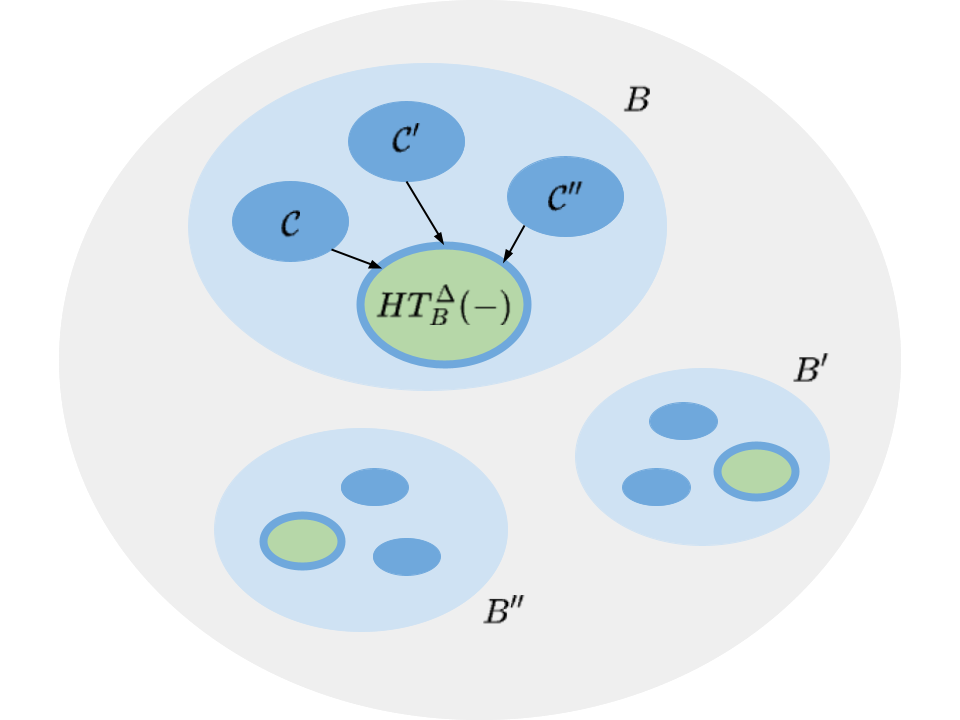
\includegraphics[width=4.5in]{intuition.png}
    \caption{\\We have some set of well-typed terms expressible in System F, which are represented by the gray circle. The terms are subdivided according to their type, and we group all terms of the same type together in the light-blue circles. For each type $B$, we have candidates $\mathcal{C}$ for type $B$, represented by the dark blue circles. \\ \\ Notice that by representing candidates, which are sets of terms, inside types, which are set of terms, we are implicitly describing type candidates as elements of a power set. \\ \\ By \Cref{lem:ht-candidate}, $\HT[B]^{\Delta}(-)$ is a type candidate. So, for every type $B$, $\HT[B]^{\Delta}(-)$ is one of the dark blue circles. These particular candidates are highlighted in green. If we can show that all well-defined terms of type $B$ are hereditarily terminating at type $B$, then we know that every element from a type candidate $C$ for type $B$ is hereditarily terminating, so $C$ is a subset of the green circle.}
    \label{fig:intuition}
\end{figure}


\paragraph{Remark.} By \Cref{lem:ht-candidate}, $\HT[B]^{\Delta}(-)$ is a type candidate. So, $\HT[B]^{\Delta}(-)$ is an option for the type candidate $\mathcal{C}$ associated with a type variable. In other words, it is one of the options for instantiating the claim ``for all candidates $\mathcal{C}$ for $B$" in the definition of hereditary termination.

\section{The Fundamental Theorem}
Now, we are almost ready to show that all well-typed terms are hereditarily terminating according to our new definition. We will require one more lemma:

\begin{lemma}[Compositionality]\label{lem:ht-comp}
    $\HT[\Sub{B}{X}{A}]^{\Delta} (M) [\eta \subseteq \delta] $ iff \\ $\HT^{\Delta,X}(M)[\eta[x \mapsto \HT[B]^{\Delta}(-)[\eta \subseteq \delta]] \subseteq \delta[x \mapsto B]]$
\end{lemma}
\begin{proof}
    By induction on the structure of $A$.
\end{proof}

We also need to redefine the notation $\Gamma \gg_\Delta M \in A$ to account for the new definition of hereditary termination, which is now defined relative to an assignment of type candidates to type variables.

\begin{definition}
    ($\HT[\Gamma]^{\Delta}(\gamma)[\eta \subseteq \delta]$)
    For all variables in $\Gamma$, if $\Gamma \entails{\isOfTp{x}{B}}$ then $\HT[B]^{\Delta}(\widehat{\gamma}(x))$
\end{definition}

\begin{definition}[$\Gamma \gg_\Delta M \in A$]
    For all substitution of type variables $\delta : \Delta$, and for all assignments of type candidates to type variables $\eta \subseteq \delta$, if $\HT[\Gamma]^{\Delta}(\gamma)[\eta \subseteq \delta]$ then $\HT^{\Delta}(\widehat{\gamma}(\widehat{\delta}(M)))[\eta \subseteq \delta]$
\end{definition}

\begin{theorem}[Fundamental Theorem]\label{thm:fundamental}
    If $\Gamma \entails[\Delta]{\isOfTp{M}{A}}$ then $\Gamma \gg_{\Delta} M \in A$.
\end{theorem}

\begin{proof}
    The proof is by induction on the derivation of $\Gamma \entails[\Delta]{\isOfTp{M}{A}}$. Here, we will consider only the cases involving type variables. The remaining cases should be standard.
    \begin{enumerate}
        \item [Rule \ruleref{sta:lam}] We can show this by instantiating type $B$ for $X$ in the premise of the rule.

        \item [Rule \ruleref{sta:app}] The Induction Hypothesis gives $\Gamma \gg_\Delta M \in \allTy*{X}{A}$ which means that for some type variable substitutions $\delta$ and term variable substitution $\gamma$, $\widehat{\gamma} (\widehat{\delta}(M)) \in \HT[\allTy*{X}{A}]^\Delta$

        Using the definition of hereditary termination, consider type $B$ and candidate $\HT[B](-)$. Then we can apply compositionality to show the desired result.
    \end{enumerate}

\end{proof}

\begin{corollary}
    A closed, well-typed term of type $\ansTy*$ is hereditarily terminating at type $\ansTy*$, which means it terminates with a value.
\end{corollary}
\end{document}
